\chapter{Unranking Restricted Permutations}
\label{cha:UnrankingMenage}

% %%%%%%%%%%%%%%%%%%%%%%%%%%%%%%%%%%%%%%%%%%%%%
% Section 1
% %%%%%%%%%%%%%%%%%%%%%%%%%%%%%%%%%%%%%%%%%%%%%
\section{Overview and history}

In January 2020, Richard Arratia sent out an email announcing a talk he was
going to give on de-ranking derangements.

By January 2021, he announced a \$100 prize for solving the analogous problem
with m\'enage permutations. I solved that too.

Richard was interested in a more general question, which I found contagious:
Given some family of combinatorial objects that can be quickly counted
(say unlabelled simple graphs on $n$ vertices)
and some total ordering on them,
when is it possible to \textbf{unrank} the collection in some computationally
efficient way?

\begin{definition}
  Let $\mathcal C$ be a totally ordered finite set, and
  let $\{c_i\}_{i=1}^{|\mathcal C|}$ be the unique sequence of elements in
  $\mathcal{C}$ such that $c_i < c_{i+1}$ for all $1 \leq i < |\mathcal{C}|$.

  The \textbf{ranking map} is the map
  $\operatorname{rank}_{\mathcal{C}} \colon \mathcal{C} \rightarrow \mathbb N_{>0}$
  which sends $c_i \mapsto i$.

  The \textbf{unranking map} is the inverse map
  $\operatorname{unrank}_{\mathcal{C}} \colon \mathbb N_{>0} \rightarrow \mathcal{C}$
  which sends $i \mapsto c_i$.
\end{definition}

In abstract terms, these maps are not particularly interesting, but in practical
terms it can be quite difficult to efficiently compute a given ranking or
unranking from a given totally ordered set. After all, when these sets
grow in exponential time or worse, explicitly constructing the sequence and
doing a search is not computationally feasible.

In Appendix \ref{apndx:unranking}, we will provide examples of total orders on combinatorial
objects $\mathcal{C}$ for which constructing efficient

% Of course, we can usually create an algorithm to give the $i$-th object without
% simply enumerating all of the objects explicitly? We want to ``jump in'' to a
% specific place on the list. Another interesting question:
% what if you get to supply both the total order and the unranking algorithm?

In this chapter we're going to explore that idea. We're going to show a general
theory that allows us to de-rank
permutations in lexicographic order,
derangements in lexicographic order,
partitions and compositions of $n$ in lexicographic order,
labeled trees by lexicographic order of Pr\"ufer code,
Lyndon words \cite{Kociumaka2014} (de Bruijn Sequences?),
Dyck path in lexicographic order?
% %%%%%%%%%%%%%%%%%%%%%%%%%%%%%%%%%%%%%%%%%%%%%
% Section 2
% %%%%%%%%%%%%%%%%%%%%%%%%%%%%%%%%%%%%%%%%%%%%%
\section{Prefix counting and word ranking}

% If we can efficiently count how many objects in
% $[n]^k$ start with a given prefix
% (in $O(T(n,k))$ time),
% then we can just walk down the possible letters until
% we get to the right spot ($O(nkT(n,k))$).

\begin{proposition}
  If we have
  an efficient way to compute the unranking map,
  an efficient way to compare two elements in the total order,
  and an efficient way of computing the number of objects at hand, $|\mathcal C|$,
  then we can efficiently compute the ranking map.
  \label{prop:unrankToRank}
\end{proposition}
\begin{proof}
  The assumptions of the proposition are enough to perform a binary search
  over $\mathcal C$, which will contribute a factor of at worst
  $\log(|\mathcal C|)$ to the running time.
\end{proof}

\subsection{Counting words with a given prefix}
In both the case of unranking derangements and menage permutations
(and in many other applications) our combinatorial objects are
words and our total order is lexicographic order, which is the extension of
alphabetical order.

\begin{definition}
  A finite \textbf{word} $w$ over an alphabet $\mathcal A$ is a finite sequence
  $\{w_i \in \mathcal A\}_{i=1}^N$.

  The collection of finite words over the alphabet $\mathcal A$ is denoted by
  $\mathcal{W}_\mathcal{A}$, or just $\mathcal{W}$ when the alphabet is
  implicit from context.
\end{definition}

\begin{definition}
  A word $w = \{w_i \in \mathcal A\}_{i=1}^N$ is said to begin with a
  \textbf{prefix} $\alpha = \{\alpha_i \in \mathcal A\}_{i=1}^M$ if
  $M \leq N$ and $w_i = \alpha_i$ for all $i \leq M$.
\end{definition}

\begin{definition}
  A word $w$ is said to be before $w'$ in lexicographic order
  if either $w$ is a proper prefix of $w'$, or if at the first position, $i$,
  where $w$ and $w'$ differ, $w_i < w'_i$.
\end{definition}

\begin{lemma}
  Let $\mathcal{W}$ be the set of words of any length on the alphabet $[n]$,
  and let $\mathcal C \subsetneq \mathcal{W}$ be a finite subset of words
  on this alphabet, with a total order equal to its lexicographic order.

  Then let
  $\#\operatorname{prefix}_{\mathcal C}\colon \mathcal{W} \rightarrow \mathcal{C}$
  be the function that counts the number of words in $\mathcal C$ that begin
  with a given prefix.

  Then the unranking function can be computed recursively by \[
    \operatorname{unrank}_\mathcal{C}(i) = f^{\mathcal C}_i((1), 0)
  \] where
  \begin{numcases}{f^{\mathcal C}_i(\alpha, j) =}
  \alpha
    & $\alpha \in \mathcal{C}$ and $i = j + 1$
  \label{case:unrankFinish}
  \\
  f^{\mathcal C}_i(\alpha', j)
    & $\alpha \not\in \mathcal{C}$ and $i \in (j, j + \#\operatorname{prefix}_\mathcal{C}(\alpha)]$
  \label{case:unrankAppend}
  \\
  f^{\mathcal C}_i(\alpha'', j + \#\operatorname{prefix}_\mathcal{C}(\alpha))
    & otherwise,
  \label{case:unrankIncrement}
  \end{numcases}
where
$\alpha = (\alpha_1, \alpha_2, \dots, \alpha_\ell)$,
$\alpha' = (\alpha_1, \alpha_2, \dots, \alpha_\ell, 1)$,
$\alpha'' = (\alpha_1, \alpha_2, \dots, \alpha_{\ell-1}, 1 + \alpha_\ell)$,
and $j$ denotes the number of words in $\mathcal{C}$ that occur strictly
before $\alpha$.
\label{lemma:unrankFromPrefix}
\end{lemma}
\begin{proof}
  We will start by inductively showing that $j$ the number of words in
  $\mathcal{C}$ that occur strictly before $\alpha$.
  The base case is clear: $0$ words occur strictly before $\alpha = (1)$,
  because $1$ is the lexicographically earliest nonempty word.

  In Equation \ref{case:unrankAppend}, $\alpha'$ is $\alpha$ with a $1$
  appended. Since $1$ is a minimal element and $\alpha \not\in \mathcal{C}$,
  there are the same number of words preceding $\alpha$ as there are preceding
  $\alpha'$.

  In Equation \ref{case:unrankIncrement}, the words that strictly precede
  $\alpha''$ are the words that precede $\alpha$, plus the words that begin
  with $\alpha$, namely $j + \#\operatorname{prefix}_\mathcal{C}(\alpha)$ of
  them.

  Now, we go case by case in showing that the recursive behavior is correct.

  To start, if $\alpha \not\in \mathcal{C}$, but
  $i \in (j, j + \#\operatorname{prefix}_\mathcal{C}(\alpha)]$,
  the range of indices of words that have prefix $\alpha$, then the known letters
  of $\alpha$ are the prefix, and so we must add on more letters to determine
  the rest of the $i$-th word.

  Otherwise we know that $i$ is not in the range of indices with that starting
  prefix so we must increment the last letter in the prefix.

  Lastly, if $\alpha \in \mathcal{C}$ and $i = j + 1$, then there are
  $j$ words preceding $\alpha$, so $\alpha$ is the $i$-th word, as desired.
\end{proof}

This shows that if we can construct a function
$\#\operatorname{prefix}_\mathcal{C}$ that efficiently counts the number of
elements of $\mathcal{C}$ with a given prefix, then we can efficiently rank and
unrank the elements of $\mathcal{C}$ in lexicographic order.
% This technique works when we can write our objects as a word in $[n]^k$, and
% we order the objects
% by the lexicographic order of the words. In the case that our objects cannot be
% written as words, or we are interested in an order other than lexicographic order,
% a different technique must be used.

\subsection{Ranking words}
In Proposition \ref{prop:unrankToRank}, we showed that given an efficient algorithm
to compute $\operatorname{unrank}_\mathcal{C}$, we can derive an efficient
algorithm to compute $\operatorname{rank}_\mathcal{C}$.

It is worth noting, however, that we can produce a more efficient algorithm,
by ranking the given word recursively.
In particular, we can say
${\operatorname{rank}_\mathcal{C}(w) = g_w(1,1,0)}$ where
\begin{equation}
  g_w(i, \ell, c) = \begin{cases}
    c + 1 & \ell = w_i \text{ and } i = |w| \\
    g_w(i + 1, 1, c) & \ell = w_i \text{ and } i < |w| \\
    g_w(i, \ell + 1, c + \#\operatorname{prefix}_\mathcal{C}(w')) & \ell < w_i,
  \end{cases}
\end{equation}
where $w' = (w_1, w_2, \dots, w_{i-1}, \ell)$.

\section{Basic notions of rook theory}
Now that we have showed that we can unrank words if we can compute the number of
words with a given prefix, we must develop techniques for this new counting
problem.
In the case of unranking derangements and permutations, it is useful to use
ideas from rook theory, which provides a theory for understanding
position-restricted permutations.
Rook Theory was introduced by Kaplansky and Riordan \cite{Kaplansky1946}
in their 1946 paper \textit{The Problem of the Rooks and its Applications}. In
it, they discuss problems of restricted permutations in the language of rooks
placed on a chessboard.

\begin{figure}
  \center
  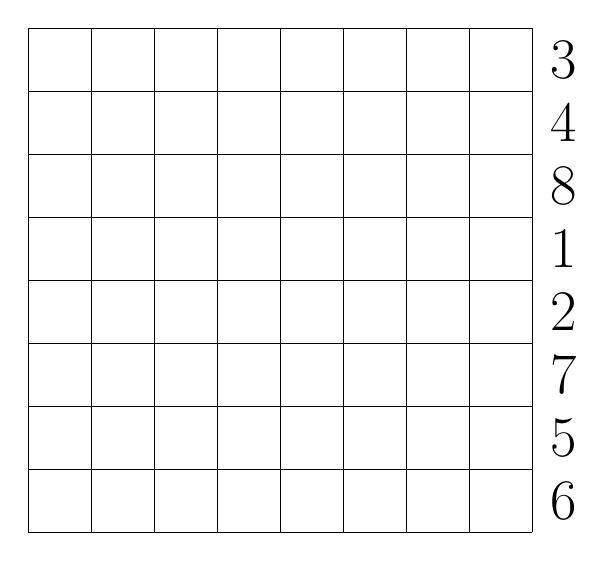
\begin{tikzpicture}[scale = 0.8]
    \foreach \i/\j in {1/3,2/4,3/8,4/1,5/2,6/7,7/5,8/6} {
      \node at (\j - 0.5, 8.5 - \i) {\huge\symrook};
      \node at (8.5, 8.5-\i) {\huge\j};
    }
    \draw (0,0) grid (8,8);
  \end{tikzpicture}
  \caption[A permutation corresponding to a rook placement.]{
    An illustration of the rook placement corresponding to the permutation
    $34812756 \in S_8$. A rook is placed in square $(i, \pi(i))$ for each $i$.
  }
  \label{fig:permutationFromRooks}
\end{figure}


\subsection{Definitions in rook theory}
We begin by introducing some preliminary ideas from rook theory.

\begin{definition}
  A \textit{board} $B$ is a subset of $[n] \times [n]$ which represents the
  squares of a $n \times n$ chessboard that rooks are allowed to be placed on.
  Every board $B$ has a \textit{complementary board}
  $B^c = ([n] \times [n]) \setminus B$, which consists of all of the
  squares of $B$ that a rook cannot be placed on.
\end{definition}

To each board, we can associate a generating polynomial that keeps track of the
number of ways to place a given number of rooks on the valid squares in such a
way that no two rooks are in the same row or column.

\begin{definition}
  The \textit{rook polynomial} associated with a board $B$,
  \[
    p_B(x) = r_0 + r_1 x + r_2 x^2 + \dots + r_n x^n,
  \]
  is a generating polynomial where $r_k$ denotes the number of $k$-element subsets
  of $B$ such that no two elements share an $x$-coordinate or a $y$-coordinate.
\end{definition}

In the context of permutations, we're typically interested in $r_n$, the number
of ways to place $n$ rooks on a restricted $n \times n$ board.
However, it turns out that a naive application of the techniques from
rook theory do not immediately allow us to count the number of
restricted permutations with a given prefix.
Computing the number of such permutations is known to be computationally hard
for a board with arbitrary restrictions.
We can see this by encoding a board $B$ as a $(0,1)$-matrix and computing the matrix
permanent. (In fact, Shevelev \cite{Shevelev1992} claims that
``the theory of enumerating the permutations with restricted positions
stimulated the development of the theory of the permanent.'')

\begin{lemma}
  Let $M_B = \{a_{ij}\}$ be an $n \times n$ matrix where \[
    a_{ij} = \begin{cases}
      1 & (i,j) \in B \\
      0 & (i,j) \not\in B
    \end{cases}.
  \]
  Then the coefficient of $x^n$ in $p_B(x)$ is given by the matrix permanent
  \[
    \operatorname{perm}(M_B) = \sum_{\sigma \in S_n} \prod_{i=1}^n a_{i\sigma(i)}.
  \]
\end{lemma}

Now is an appropriate time to recall Valiant's Theorem.

\begin{theorem}[Valiant's Theorem \cite{Valiant1979}]
  The counting problem of of computing the permanent of a (0,1)-matrix is \#P-complete.
\end{theorem}

\begin{corollary}
  Computing the number of rook placements on an arbitrary $n \times n$ board is
  \#P-hard.
\end{corollary}

Therefore, in order to compute the number of permutations, we must exploit some
additional structure of the restrictions.

\subsection{Techniques of rook theory}
Rook polynomials can be computed recursively. The base case is that
for an empty board $B = \emptyset$, the corresponding rook polynomial is
$p_\emptyset(x) = 1$, because there is one way to place no rooks, and no way
to place one or more rooks.
\begin{lemma}[\cite{Riordan1980}]
  Given a board, $B$, then for any square $(x,y) \in B$, we can define
  the resulting boards if we include or exclude the square respectively
  \begin{align}
    B_i &= \{(x',y') \in B : x \neq x' \text{ and } y \neq y'\} \\
    B_e &= B \setminus {(x,y)}.
  \end{align}
  Then we can write the rook polynomial for $B$ in terms of this decomposition.
  \[
    p_B(x) = xp_{B_i}(x) + p_{B_e}(x).
  \]
  \label{lemma:rookPolynomialRecursion}
\end{lemma}

If we want to compute a rook polynomial using this construction, we can end
up adding up lots of smaller rook polynomials---a number that is exponential in
the size of $B$.
However, when the number of squares in $B^c$ is small in some sense, it can be
easier to compute the rook polynomial $p_{B^c}$ and use the principle of
inclusion/exclusion on it's coefficients to determine the rook polynomial for
the original board, $B$.

In the case of derangements and m\'enage permutations, this is the strategy
we'll use.
Start by finding the resulting board from a given prefix,
find the rook polynomial of the complementary board, and
use the principle of inclusion/exclusion to determine the number of ways to
place rooks in the resulting board.

\section{Unranking derangements}

In January 2020, Richard Arratia sent out an email proposing a seminar talk.
The title describes the first ``\$100 problem'':
\begin{problem}
``For $100$ dollars, what is the $500$ quadrillion-th derangement on $n=20$?''
\end{problem}

\begin{answer}
The computer program in Appendix \ref{apndx:haskell} computed the answer in less than ten
milliseconds. When written as words in lexicographic order, the
derangement in $S_{20}$ with rank $5 \times 10^{17}$ is \[
  12\ 14\ 2\ 9\ 13\ 20\ 6\ 3\ 1\ 17\ 5\ 11\ 19\ 15\ 10\ 18\ 8\ 7\ 4\ 16.
\]
\end{answer}

Arratia's question focused on unranking derangements where the rank was
based on the total ordering that comes from writing the
permutations as words in lexicographic order.
Other authors have looked at unranking derangements based on other total
orderings. In particular, Mikawa and Tanaka \cite{Mikawa2014} give an algorithm
to rank/unrank derangements
with respect to \textit{lexicographic ordering in cycle notation}.

In this section we will develop an algorithm for ranking and unranking with
respect to their lexicographic ordering as words. The technique that we use will
broadly be re-used in the next section.
It is worthwhile to begin by recalling the definition of a derangement.
\begin{definition}
  A \textit{derangement} is a permutation $\pi \in S_n$ such that $\pi$ has no
  fixed points. That is, the set of derangements on $n$ letters is \[
    \mathcal{D}_n = \{\pi \in S_n : \pi(i) \neq i\ \forall i \in [n]\}.
  \]
\end{definition}

\subsection{The complementary board}
In order to compute the number of derangements with a given prefix, it is
useful to look at the board that results after placing $k$ rooks according to
these positions, as illustrated in Figure \ref{fig:derangementPrefix}.

\begin{figure}
  \center
  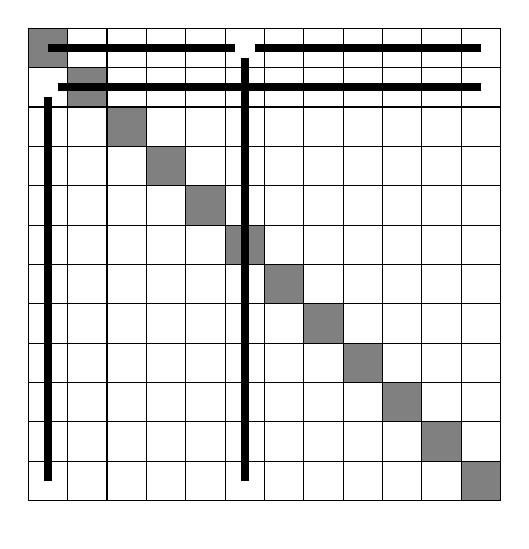
\begin{tikzpicture}[scale = 0.5]
    \path (0,-0.5) -- (0,6.5);
    \foreach \i in {0,...,11} { \fill[gray] (\i, 12-\i) rectangle (\i + 1, 11 - \i); }
    \draw (0,0) grid (12,12);
    \node (R1) at (5.5, 11.5) {\Large\rook};
    \node (R2) at (0.5, 10.5) {\Large\rook};
    \draw[line width = 3]
      (0.5,11.5) -- (R1) -- (11.5,11.5)
      (R1) -- (5.5,0.5)
    ;
    \draw[line width = 3]
      (R2) -- (11.5,10.5)
      (R2) -- (0.5,0.5)
    ;
  \end{tikzpicture}
  ~~
  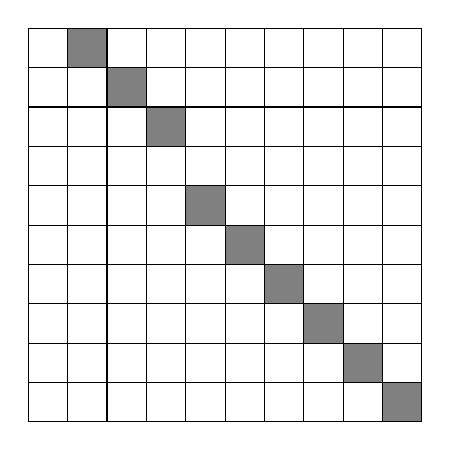
\begin{tikzpicture}[scale = 0.5]
    \path (0,-0.5) -- (0,6.5);
    \foreach \i in {1,...,3} { \fill[gray] (\i, 11-\i) rectangle (\i + 1, 10 - \i); }
    \foreach \i in {4,...,9} { \fill[gray] (\i, 10-\i) rectangle (\i + 1, 9 - \i); }
    \draw (0,0) grid (10,10);
  \end{tikzpicture}
  \caption[The derived board for a prefix of a derangement.]{An example of a prefix $\alpha = (6, 1)$, and the board that results
  from deleting the first $\ell = 2$ rows and columns $6$ and $1$.
  The derived complementary board of $B$ from $\alpha$ is
  $B^c_\alpha = \{(1,2), (2,3), (3,4), (5,5), \dots, (10,10)\}$.}
\label{fig:derangementPrefix}
\end{figure}


\begin{definition}
  If $B$ is an $n \times n$ board, and
  $\alpha = (\alpha_1, \alpha_2, \dots, \alpha_\ell)$ is a valid prefix of length
  $\ell$, then \textbf{derived board} of $B$ from $\alpha$,
  denoted $B_\alpha$,
  is constructed by removing
  rows $1, 2, \dots, \ell$ and
  columns $\alpha_1, \alpha_2, \dots, \alpha_ell$ from $B$,
  reindexing in such a way that both the row and column indexes are in
  $[n - \ell]$.

  The \textbf{derived complementary board} $B_\alpha^c$ is the complement of
  $B_\alpha$ with respect to $[n - \ell] \times [n - \ell]$.
\end{definition}

Given a prefix of length $\ell$, the number of ways of placing $n - \ell$ rooks
on the derived board $B_\alpha$ is, by construction,
equal to the number of words in $\mathcal{C}$ with prefix $\alpha$
\begin{lemma}
  Given a valid $\ell$ letter prefix $(\alpha_1, \alpha_2, \dots, \alpha_\ell)$
  of a word on $n$ letters,
  the number of squares in the derived complementary board is \[
    |B_\alpha^c| = n - \ell - |\{\ell+1, \ell+2, \dots, n\} \cap \{\alpha_1, \alpha_2, \dots, \alpha_\ell\}|,
  \] and no two of these squares are in the same row or column.
  \label{lemma:derangementComplementSize}
\end{lemma}
\begin{proof}
  Notice that the derived complementary board can be constructed in a different
  order: by first taking the complement, then deleting rows and columns, and
  finally reindexing the squares.
  Because, the complementary board has no two squares in the same row or column,
  deleting and reindexing results in a derived complementary board with the same
  property.

  Thus, we only need to classify which squares in the complementary board are
  deleted to make the derived complementary board.
  We start by deleting $\ell$ squares corresponding to the deletion of the first
  $\ell$ rows, namely $(1, 1), (2, 2), \dots, (\ell, \ell)$.

  Some of these squares may also be in columns
  $\alpha_1, \alpha_2, \dots, \alpha_\ell$, but to avoid double-counting, we
  only consider those letters that are greater than $\ell$. These are
  $|\{\ell+1, \ell+2, \dots, n\} \cap \{\alpha_1, \alpha_2, \dots, \alpha_\ell\}|$,
  as desired.
\end{proof}

\subsection{Derangements with a given prefix}
Now that we have a way of quickly computing $|B_\alpha^c|$, we can compute the
number of ways to place a given number of rooks on the complementary board.
We can use this
to compute the rook polynomial for the derived complementary board
$p_{B_\alpha^c}(x)$.
We will see later that we can use the coefficients of this polynomial to compute
the number of ways of placing $n - \ell$ rooks on the derived board $B_\alpha$.

\begin{lemma}
  The rook polynomial for the complementary board $B_\alpha^c$ is \begin{equation}
    p_{B_\alpha^c}(x) = \sum_{j = 0}^{|B_\alpha^c|} \binom{|B_\alpha^c|}{j}x^j.
  \end{equation}
\end{lemma}
\begin{proof}
  Recall that no two squares of $B^c_\alpha$ are in the same row or column.
  Thus the number of ways to place $j$ rooks is equivalent to selecting any
  $j$ squares from the collection of $|B^c_\alpha|$ squares.

  Therefore the coefficient of $x^j$ in the rook polynomial is
  $\binom{|B_\alpha^c|}{j}$.
\end{proof}

Now we introduce a lemma of Stanley \cite{Stanley2011EC1} to compute the number
of ways of placing $n - \ell$ rooks in a complementary board
$B_\alpha \subseteq [n - \ell] \times [n - \ell]$.

\begin{lemma}[\cite{Stanley2011EC1}]
  Let $B \subseteq [n] \times [n]$ be a board with complementary board $B^c$,
  and denote the rook polynomial of $B^c$ by
  $P_{B^c}(x) = \sum_{k=0}^n r^c_k x^k$.

  Then the number of ways, $N_0$, of placing $n$ nonattacking rooks on $B$
  is given by the principle of inclusion/exclusion
  \[
    N_0 = \sum_{k=0}^n (-1)^k r^c_k (n-k)!.
  \]
  \label{lemma:CountsFromComplementaryPolynomials}
\end{lemma}

This lemma allows us to compute rook placements on the derived board $B_\alpha$,
which is the number of derangements in $\mathcal{D}$ that begin with the prefix
$\alpha$.
\begin{corollary}
  The number of derangements with prefix
  $\alpha = (\alpha_1, \alpha_2, \dots, \alpha_\ell)$
  is given by \[
    \#\operatorname{prefix}_\mathcal{D}(\alpha)
    = \sum_{j=0}^{|B_\alpha^c|} (-1)^j \binom{|B_\alpha^c|}{j}(n-\ell-j)!,
  \] which is $\operatorname{A047920}(n-\ell, |B_\alpha^c|)$ in
  the On-Line Encyclopedia of Integer Sequences (OEIS) \cite{oeis}.
\end{corollary}

Because we can compute $|B_\alpha^c|$ from $\alpha$ in linear time
(see Lemma \ref{lemma:derangementComplementSize}), if we use a computational
model where factorials are given by an oracle and arithmetic can be computed
in constant time, then $\#\operatorname{prefix}_\mathcal{D}$ can be computed
in linear time with respect to $\ell$, the length of the prefix.

\begin{example}
  For example, for $n = 14$, we wish to count the number of derangements that
  start with the prefix $\alpha = (6,1)$.
  Since the prefix has two letters, $\ell = 2$ and $n - \ell = 14 - 2 = 12$.
  Number of squares in $B_\alpha^c$ is \[
    |B_\alpha^c| = 14 - 2 - \underbrace{|\{3,4,\dots,14\} \cap \{6, 1\}|}_1 = 11
  \]
  Thus there are $A047920(12,11) = 190\,899\,411$ derangements that start
  with $\alpha = (6,1)$.
\end{example}

Now that we have an efficient algorithm for computing
$\#\operatorname{prefix}_\mathcal{D} \colon \mathcal{W} \rightarrow \mathbb{N}_{\geq 0}$,
we can invoke the recursive formula in Lemma \ref{lemma:unrankFromPrefix} to
compute
$\operatorname{unrank}_\mathcal{D} \colon \mathbb{N}_{\geq 0} \rightarrow \mathcal{D}$
and unrank derangements.
The sequence of recursive steps is illustrated in
Table \ref{table:unrankDerangement}.
\begin{table}
\center
\begin{tabular}{|l|r|l|c|l|}
  \hline
  $\alpha$ (prefix)
    & $\operatorname{\#prefix}_\mathcal{D}(\alpha)$
    & index range
    & $|B_\alpha^c|$
    & $\operatorname{unrank}_\mathcal{D}(1000)$
  \\ \hline
  $1       $ & $0$    & $(0,0]$           & $-$ & $f^{\mathcal{D}}_{1000}(1, 0)$          \\
  $2       $ & $2119$ & $(0,2119]$        & $6$ & $f^{\mathcal{D}}_{1000}(2, 0)$          \\
  \hline
  $21      $ & $265$  & $(0, 265]$        & $6$ & $f^{\mathcal{D}}_{1000}(21, 0)$         \\
  $22      $ & $0$    & $(265, 265]$      & $-$ & $f^{\mathcal{D}}_{1000}(22, 265)$       \\
  $23      $ & $309$  & $(265, 574]$      & $5$ & $f^{\mathcal{D}}_{1000}(23, 265)$       \\
  $24      $ & $309$  & $(574, 883]$      & $5$ & $f^{\mathcal{D}}_{1000}(24, 574)$       \\
  $25      $ & $309$  & $(883, 1192]$     & $5$ & $f^{\mathcal{D}}_{1000}(25, 883)$       \\
  \hline
  $251     $ & $53$   & $(883, 936]$      & $4$ & $f^{\mathcal{D}}_{1000}(251, 883)$      \\
  $253     $ & $0$    & $(936, 936]$      & $-$ & $f^{\mathcal{D}}_{1000}(253, 936)$      \\
  $254     $ & $64$   & $(936, 1000]$     & $3$ & $f^{\mathcal{D}}_{1000}(254, 936)$      \\
  \hline
  $2541    $ & $11$   & $(936, 947]$      & $3$ & $f^{\mathcal{D}}_{1000}(2541, 936)$     \\
  $2543    $ & $11$   & $(947, 958]$      & $3$ & $f^{\mathcal{D}}_{1000}(2543, 947)$     \\
  $2546    $ & $14$   & $(958, 972]$      & $2$ & $f^{\mathcal{D}}_{1000}(2546, 958)$     \\
  $2547    $ & $14$   & $(972, 986]$      & $2$ & $f^{\mathcal{D}}_{1000}(2547, 972)$     \\
  $2548    $ & $14$   & $(986, 1000]$     & $2$ & $f^{\mathcal{D}}_{1000}(2548, 986)$     \\
  \hline
  $25481   $ & $3$    & $(986, 989]$      & $2$ & $f^{\mathcal{D}}_{1000}(25481, 986)$    \\
  $25483   $ & $3$    & $(989, 992]$      & $2$ & $f^{\mathcal{D}}_{1000}(25483, 989)$    \\
  $25486   $ & $4$    & $(992, 996]$      & $1$ & $f^{\mathcal{D}}_{1000}(25486, 992)$    \\
  $25487   $ & $4$    & $(996, 1000]$     & $1$ & $f^{\mathcal{D}}_{1000}(25487, 996)$    \\
  \hline
  $254871   $ & $2$   & $(996, 998]$      & $0$ & $f^{\mathcal{D}}_{1000}(254871, 996)$   \\
  $254873   $ & $2$   & $(998, 1000]$     & $0$ & $f^{\mathcal{D}}_{1000}(254873, 998)$   \\
  \hline
  $2548731  $ & $1$   & $(998, 999]$      & $0$ & $f^{\mathcal{D}}_{1000}(2548731, 998)$  \\
  $2548736  $ & $1$   & $(999, 1000]$     & $0$ & $f^{\mathcal{D}}_{1000}(2548736, 999)$  \\
  \hline
  $25487361 $ & $1$   & $(999, 1000]$     & $0$ & $f^{\mathcal{D}}_{1000}(25487361, 999)$ \\
  \hline
\end{tabular}
\caption[Steps for computing the $1000$th derangement in $S_8$]{
  There are $A000166(8) = 14833$ derangements on $8$ letters.
  The table shows the recursive steps to find that the derangement at index
  $1000$ is $25487361$.
}
\label{table:unrankDerangement}
\end{table}

% %%%%%%%%%%%%%%%%%%%%%%%%%%%%%%%%%%%%%%%%%%%%%
% Section 3
% %%%%%%%%%%%%%%%%%%%%%%%%%%%%%%%%%%%%%%%%%%%%%
\section{Unranking m\'enage permutations}
\label{sec:unrankingMenage}
After claiming a prize for unranking derangements, the conversation shifted to
how this technique could be extended. A natural next step seemed to be to look
at another family of restricted permutations, namely m\'enage permutations.

A m\'enage permutation comes from the \textit{probl\`eme des m\'enages},
introduced by \'Edouard Lucas in 1891.
There are a few choices of how to define these permutations, but we will
use the following definition for simplicity.
\begin{definition}
  A \textit{m\'enage permutation} is a permutation $\pi \in S_n$ such that for
  all $i \in [n]$,
  $\pi(i) \neq i$ and
  $\pi(i) + 1 \not\equiv i \bmod n$.
  The set of m\'enage permutations of length $n$ is denoted $\pazocal{M}_n$.
\end{definition}

\subsection{Proof of concept (the \$100 answer!)}
By February 2020, it appeared that the techniques for unranking derangements
would not directly translate to the context of m\'enage permutations. In
response, Richard Arratia upped the stakes, offering another prize for
unranking m\'enage permutations. Specifically, he posed the following problem.
\begin{problem}
  For $n=20$ there are $A000179(20) = 312\,400\,218\,671\,253\,762 > 3.1\cdot 10^{17}$
  m\'enage permutations.
  Determine the $10^{17}$-th such permutation when listed in lexicographic order.
\end{problem}
Using the techniques described in this section, we developed a computer program that
computed the answer in less than $0.03$ seconds.
(By comparison, unranking the $10^{157}$-th m\'enage permutation of the more
than $1.25 \times 10^{157}$ m\'enage permutations in $S_{100}$
with the same program takes about $7$ seconds.)
\begin{answer}
  The desired permutation is \begin{equation}
    7\ 16\ 19\ 12\ 2\ 8\ 15\ 1\ 18\ 14\ 3\ 9\ 20\ 10\ 5\ 17\ 13\ 4\ 11\ 6.
  \end{equation}
\end{answer}

\subsection{Overview for unranking m\'enage permutations}

As in the section about unranking derangements, we will use the insight from
Lemma \ref{lemma:unrankFromPrefix} that if we can efficiently count the number
of words with a give prefix, then we can efficiently unrank the words.

The technique exploits the following observations:
after placing rooks on a board corresponding to our
prefix, the remaining board has the property that its complement is block
diagonal. These complementary blocks have a structure that we can understand,
and we can leverage that understanding to compute the rook polynomials of these
blocks and consequently of the complementary board itself. Once we have computed
the rook polynomial of the complementary board, we can use the principle of
inclusion/exclusion to compute the number of full rook placements on the
original board.
This gives us the number of m\'enage permutations with a given prefix.

\subsection{Disjoint board decomposition}
Looking at Figure \ref{fig:menageMultiplePlacement},
it appears that placing rooks according to a prefix
results in a board whose complement can be partitioned into
sub-boards whose squares don't share any rows or columns.
We will see that this property indeed holds in general,
and we can exploit this in order to count the m\'enage permutations
with a given prefix.

\begin{figure}[ht!]
  \center
  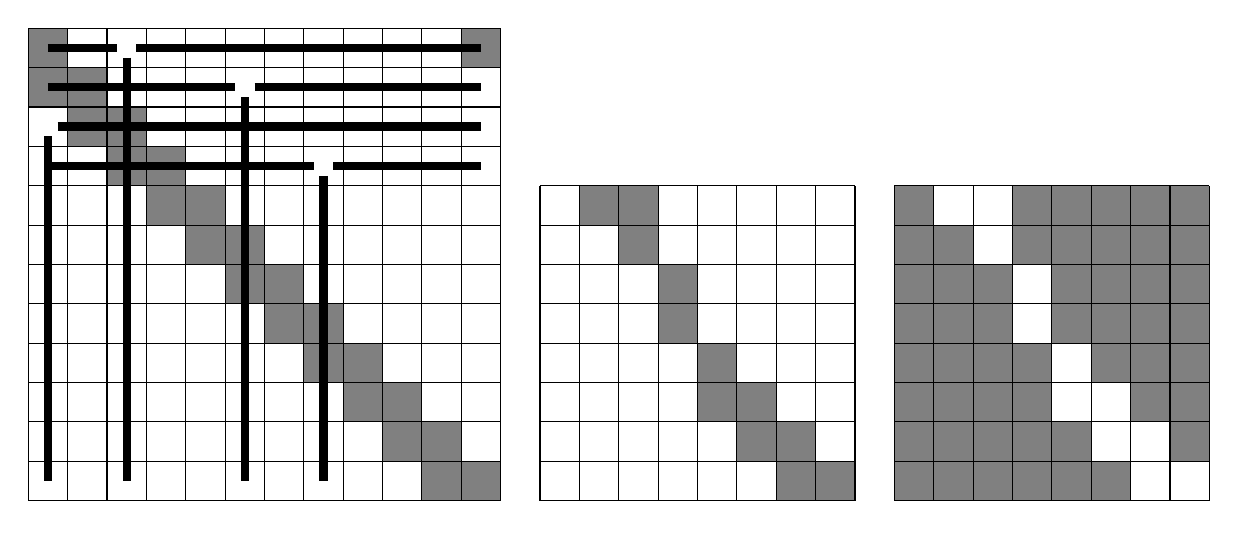
\begin{tikzpicture}[scale = 0.5]
    \path (0,-0.5) -- (0,6.5);
    \foreach \i in {0,...,11} { \fill[gray] (\i, 12-\i) rectangle (\i + 1, 11 - \i); }
    \foreach \i in {0,...,10} { \fill[gray] (\i, 11-\i) rectangle (\i + 1, 10 - \i); }
    \fill[gray] (11,11) rectangle (12,12);
    \draw (0,0) grid (12,12);
    \node (R1) at (2.5, 11.5) {\Large\rook};
    \node (R2) at (5.5, 10.5) {\Large\rook};
    \node (R3) at (0.5, 9.5) {\Large\rook};
    \node (R4) at (7.5, 8.5) {\Large\rook};
    \draw[line width = 3]
      (0.5,11.5) -- (R1) -- (11.5,11.5)
      (R1) -- (2.5,0.5)
    ;
    \draw[line width = 3]
      (0.5,10.5) -- (R2) -- (11.5,10.5)
      (R2) -- (5.5,0.5)
    ;
    \draw[line width = 3]
      (R3) -- (11.5,9.5)
      (R3) -- (0.5,0.5)
    ;
    \draw[line width = 3]
      (0.5,8.5) -- (R4) -- (11.5,8.5)
      (R4) -- (7.5,0.5)
    ;
    % ---------------------------------------------
    \foreach \i/\j in {1/7, 2/6, 2/7, 3/4, 3/5, 4/2, 4/3, 5/2, 5/1, 6/1, 6/0, 7/0} {
      \fill[gray, xshift=13cm] (\i, \j) rectangle (\i + 1, \j + 1);
    }
    \draw[xshift=13cm] (0,0) grid (8,8);
    % ---------------------------------------------
    \fill[xshift=22cm, gray] (0,0) rectangle (8,8);
    \foreach \i/\j in {1/7, 2/6, 2/7, 3/4, 3/5, 4/2, 4/3, 5/2, 5/1, 6/1, 6/0, 7/0} {
      \fill[white, xshift=22cm] (\i, \j) rectangle (\i + 1, \j + 1);
    }
    \draw[xshift=22cm] (0,0) grid (8,8);
  \end{tikzpicture}
  % ~~~
  % \begin{tikzpicture}[scale = 0.5]
  %   \path (0,-0.5) -- (0,6.5);
  %   \foreach \i/\j in {0/7, 0/6, 1/6, 1/5, 2/5, 2/4, 3/4, 4/3, 5/3, 5/2, 6/1, 6/0} {
  %     \fill[gray] (\i, \j) rectangle (\i + 1, \j + 1);
  %   }
  %   \draw (0,0) grid (8,8);
  %   \draw[ultra thick, dashed, red]
  %     (0,8) rectangle (4,4)
  %     (4,4) rectangle (6,2)
  %     (6,2) rectangle (8,0)
  %   ;
  % \end{tikzpicture}
  \caption[An example of a derived complementary board.]{
    The prefix $\alpha = (3,6,1,8)$,
    the derived board $B_\alpha$, and
    the derived complementary board
    $B_\alpha^c = \mathcal{O}_3 \sqcup \mathcal{E}_2 \sqcup \mathcal{O}_7^\intercal$.
    There are $8062$ ways of placing eight nonattacking rooks on $B_\alpha$.
  }
  \label{fig:menageMultiplePlacement}
\end{figure}


The property of complements that can be partitioned into sub-boards
whose squares don't share rows or columns is useful because it provides
a way of factoring the rook polynomial of the bigger board into the rook
polynomials of the sub-boards.
\begin{definition}
  Two sub-boards $B$ and $B'$ are called \textbf{disjoint} if no squares of $B$ are
  in the same row or column as any square in $B'$.
\end{definition}

Kaplansky gives a way of computing the rook polynomial of a board in terms of
its disjoint boards.
\begin{theorem}[\cite{Kaplansky1946}]
  If $B$ can be partitioned into disjoint boards $b_1, b_2, \dots, b_m$,
  then the rook polynomial of $B$ is the product of the rook polynomials of
  the $b_i$s \[
    p_B(x) = \prod_{i=1}^m p_{b_i}(x).
  \]
\end{theorem}

We will use this disjoint board decomposition repeatedly, because as
Figure \ref{fig:menageMultiplePlacement} suggests, the boards that result
after placing a prefix can be partitioned into disjoint sub-boards whose
structure is well understood. Now we will give a name to these blocks,
which are illustrated in Figure \ref{fig:blockShape}.

\begin{figure}[ht!]
  \center
  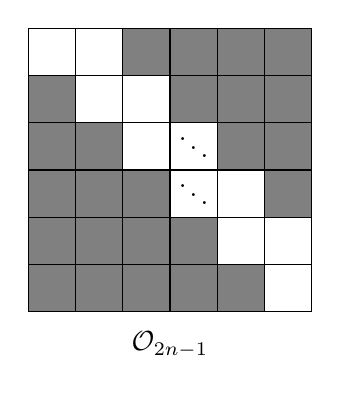
\begin{tikzpicture}[scale=0.6]
    \fill[gray] (1,0) rectangle (7,6);
    \foreach \i/\j in {1/5, 2/5, 2/4, 3/4, 3/3, 4/3, 4/2, 5/2, 5/1, 6/1, 6/0} { \fill[white] (\i, \j) rectangle (\i + 1, \j + 1); }
    \node at (4.5,3.65) {$\ddots$};
    \node at (4.5,2.65) {$\ddots$};
    \draw (1,0) grid (7,6);
    \path (1,-1.5) rectangle (7,6);
    \node at (4, -0.7) {$\mathcal{O}_{2n-1}$};
  \end{tikzpicture}
  ~
  \begin{tikzpicture}[scale=0.6]
    \fill[gray] (1,0) rectangle (7,6);
    \foreach \i/\j in {1/5, 1/4, 2/4, 2/3, 3/2, 3/3, 4/1, 4/2, 5/1, 5/0, 6/0} { \fill[white] (\i, \j) rectangle (\i + 1, \j + 1); }
    \node at (3.5,2.65) {$\ddots$};
    \node at (4.5,2.65) {$\ddots$};
    \draw (1,0) grid (7,6);
    \path (1,-1.5) rectangle (7,6);
    \node at (4, -0.7) {$\mathcal{O}_{2n-1}^\intercal$};
  \end{tikzpicture}
  ~
  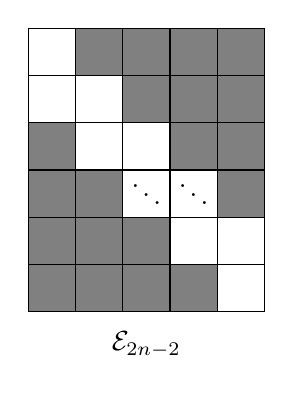
\begin{tikzpicture}[scale=0.6]
    \fill[gray] (1,0) rectangle (6,6);
    \foreach \i/\j in {1/4, 1/5, 2/3, 2/4, 3/2, 3/3, 4/1, 4/2, 5/0, 5/1} { \fill[white] (\i, \j) rectangle (\i + 1, \j + 1); }
    \node at (3.5,2.65) {$\ddots$};
    \node at (4.5,2.65) {$\ddots$};
    \draw (1,0) grid (6,6);
    \path (1,-1.5) rectangle (6,6);
    \node at (3.5, -0.7) {$\mathcal{E}_{2n-2}$};
  \end{tikzpicture}
  ~
  \begin{tikzpicture}[scale=0.6]
    \fill[gray] (1,1) rectangle (7,6);
    \foreach \i/\j in {1/5, 2/5, 2/4, 3/4, 3/3, 4/3, 4/2, 5/2, 5/1, 6/1} { \fill[white] (\i, \j) rectangle (\i + 1, \j + 1); }
    \node at (4.5,3.65) {$\ddots$};
    \node at (4.5,2.65) {$\ddots$};
    \path (1,-0.5) rectangle (7,7);
    \draw (1,1) grid (7,6);
    \node at (4, 0.3) {$\mathcal{E}_{2n-2}^\intercal$};
  \end{tikzpicture}
  \caption[Block shapes for a m\'enage permutation.]{
    Examples of each of the four staircase-shaped boards.
    The first two boards are on grids of size $n \times n$,
    the third is on a grid of size $n \times (n-1)$ and the
    fourth is on a grid of size $(n-1) \times n$.
  }
  \label{fig:blockShape}
\end{figure}


\begin{definition}
  A board is called \textbf{staircase-shaped} if it matches one of the
  following four shapes:
  \begin{alignat*}{2}
    \mathcal{O}_{2n-1}           &= \{(i,i) : i \in [n]\}    &&\cup\ \{(i,i+1) : i \in [n-1]\} \\
    \mathcal{O}_{2n-1}^\intercal &= \{(i,i) : i \in [n]\}    &&\cup\ \{(i+1,i) : i \in [n-1]\} \\
    \mathcal{E}_{2n-2}           &= \{(i,i) : i \in [n-1]\}\ &&\cup\ \{(i+1,i) : i \in [n-1]\} \\
    \mathcal{E}_{2n-2}^\intercal &= \{(i,i) : i \in [n-1]\}\ &&\cup\ \{(i,i+1) : i \in [n-1]\},
  \end{alignat*}
  the subscripts represent the number of squares, and the names represent their
  parity.
  \label{def:staircaseShaped}
\end{definition}

We now show that our resulting boards can be partitioned into boards of these shapes.

\begin{lemma}
  For $\ell \geq 1$, and prefix $\alpha = (\alpha_1, \alpha_2, \dots, \alpha_\ell)$
  the derived complementary board $B_\alpha^c$ can be partitioned into
  disjoint staircase-shaped boards.
  \label{lemma:boardShape}
\end{lemma}
\begin{proof}
  The proof proceeds by induction on the length of the prefix.

  To establish the base case, consider a prefix of length $\ell = 1$.
  Because of the m\'enage restriction,
  $\alpha_1 \in \{2, 3, \dots, n-1\}$, and
  the derived complimentary board $B_{(\alpha_1)}^c$
  can be partitioned into two disjoint sub-boards with shapes
  $A_{\alpha_1 - 1}$ and $A^\intercal_{n - \alpha_1}$.
  (This is illustrated for the case of $n = 7$ and $\alpha_1$ in
  Figure \ref{fig:menageSinglePlacement}.)

  The inductive hypothesis is that the derived complimentary board for
  a prefix of length $\ell - 1$ consists of sub-boards with shape
  $A_{n_1}$, $A^\intercal_{n_2}$, $B_{n_3}$, or $B^\intercal_{n_4}$.
  Placing a rook in row $\ell$ can remove a top row or a column or both in a
  given sub-board.
  Table \ref{table:rooksInBlocks} below
  shows the resulting sub-boards after placing a rook in
  $\ell$-th row of $B$,
  which may be in the top row or the $i$-th column of a given sub-board.
  \captionsetup{type=table}
  \begin{tabular}{|l|l|l|l|l|}
  \hline
  Rook placement
    & $\mathcal{O}_{2n-1}$
    & $\mathcal{O}_{2n-1}^\intercal$
    & $\mathcal{E}_{2n-2}$
    & $\mathcal{E}_{2n-2}$
  \\ \hline
  Row $1$
    & $\mathcal{O}_{2n-3}$
    & $\mathcal{E}_{2n-2}^\intercal$
    & $\mathcal{O}_{2n-3}$
    & $\mathcal{E}_{2n-4}^\intercal$
  \\
  Column $i$
    & $\mathcal{O}_{2i-3}$, $\mathcal{E}_{2n-2i}$
    & $\mathcal{E}_{2i-2}$, $\mathcal{O}_{2n-2i-1}^\intercal$
    & $\mathcal{E}_{2i-2}$, $\mathcal{E}_{2n-2i-2}$
    & $\mathcal{O}_{2i-3}$, $\mathcal{O}_{2n-2i-1}^\intercal$
  \\
  Row $1$, column $i$
    & $\mathcal{O}_{2i-5}$, $\mathcal{E}_{2n-2i}$
    & $\mathcal{O}_{2i-3}$, $\mathcal{O}_{2n-2i-1}^\intercal$
    & $\mathcal{O}_{2i-3}$, $\mathcal{E}_{2n-2i-2}$
    & $\mathcal{O}_{2i-5}$, $\mathcal{O}_{2n-2i-1}^\intercal$
  \\ \hline
  \end{tabular}
  \captionof{table}[Rook placements on staircase-shaped boards]{
    The results of placing a rook in the first row, $i$-th column, or both
    for all staircase-shaped boards.
  }
  \label{table:rooksInBlocks}
  Therefore placing any number of rooks in the first $\ell$ results in a board
  of one of the four described shapes.
\end{proof}

\begin{figure}[ht!]
  \center
  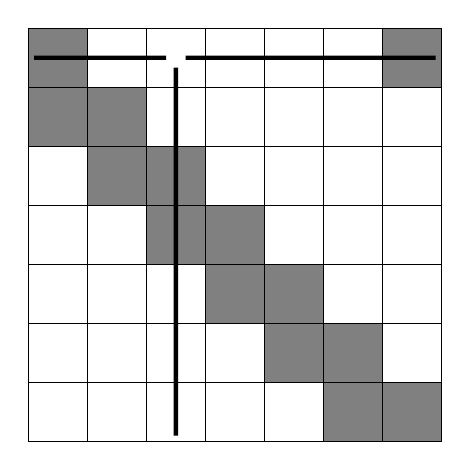
\begin{tikzpicture}[scale = 0.75]
    \foreach \i in {0,...,6} { \fill[gray] (\i, 6 - \i) rectangle (\i + 1, 7 - \i); }
    \foreach \i in {1,...,6} { \fill[gray] (\i-1, 6 - \i) rectangle (\i, 7 - \i); }
    \fill[gray] (6, 6) rectangle (7, 7);
    \draw (0,0) grid (7,7);
    \node (R) at (2.5, 6.5) {\huge\rook};
    \draw[ultra thick]
      (0.1,6.5) -- (R) -- (6.9,6.5)
      (R) -- (2.5,0.1)
    ;
  \end{tikzpicture}
  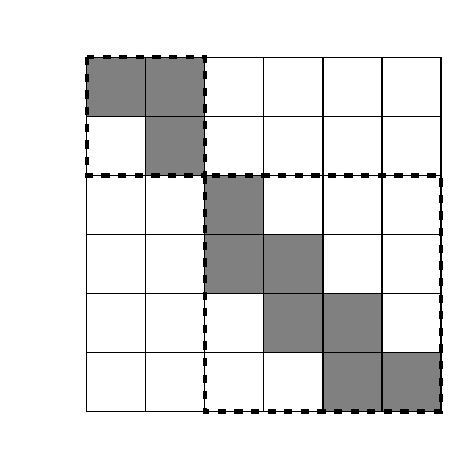
\begin{tikzpicture}[scale = 0.75]
    \path (0,-0.5) -- (0,6.5); % vertically center.
    \foreach \i/\j in {1/5, 2/5, 2/4, 3/3, 3/2, 4/2, 4/1, 5/1, 5/0, 6/0} { \fill[gray] (\i, \j) rectangle (\i + 1, \j + 1); }
    \draw[ultra thick, dashed] (1,6) rectangle (3,4) rectangle (7,0);
    \draw (1,0) grid (7,6);
  \end{tikzpicture}
  \caption[The derived board for a prefix of a m\'enage permutation of length $1$.]{
    The first chessboard shows a placement of a rook at position $3$,
    the second shows how the derived complementary board can be partitioned
    into two disjoint boards with $3$ and $7$ squares respectively.
  }
  \label{fig:menageSinglePlacement}
\end{figure}


\subsection{Rook polynomials of blocks}
Recall that the goal of partitioning $B$ into disjoint sub-boards
$b_1, b_2, \dots, b_m$ is so that we can
factor $p_B(x)$ in terms of $p_{b_i}(x)$.
Of course, this is only useful if we can describe $p_{b_i}(x)$,
which is the goal of this subsection.
Conveniently, the rook polynomial of each $b_i$ will turn out to depend only on the
number of squares, $|b_i|$, which can be computed easily because of its
staircase shape.

We will begin by defining a family of polynomials that, suggestively, will turn
out to be the rook polynomials that we are looking for.
This family is described by OEIS sequence A011973 \cite{oeis}.
\begin{definition}
  For $j \geq 0$, the $j$th \textbf{Fibonacci polynomial} $F_{j}(x)$ is defined recursively as:
  \begin{align}
    F_0(x) &= 1 \\
    F_1(x) &= 1 + x \\
    F_n(x) &= xF_{n-2}(x) + F_{n-1}(x).
  \end{align}
\end{definition}

The rook polynomials of the staircase-shaped boards agree with these Fibonacci
polynomials.

\begin{lemma}
  If $B$ is a staircase-shaped board with $k$ squares, then
  $B$ has rook polynomial $p_{B}(x) = F_{k}(x)$, equal to the $k$-th
  Fibonacci polynomial.
  \label{lemma:staircaseIsFibonacci}
\end{lemma}
\begin{proof}
  We will recall the recursive construction of rook polynomials from
  Lemma \ref{lemma:rookPolynomialRecursion}, and proceed by
  induction on the number of squares, always choosing to include or exclude
  the upper-left square.

  Since the reflections of board has the same rook polynomial as the
  unreflected board, without loss of generality, we
  will compute the rook polynomials for
  $\mathcal{O}_{2n-1}$ and $\mathcal{E}_{2n-2}$ respectively.

  To establish a base case, consider the rook polynomials when $n = 1$, so
  the even board has $|\mathcal{E}_{0}| = 0$ squares and
  the odd board has $|\mathcal{O}_{1}| = 1$ square.
  We can see the corresponding rook polynomials directly. There is $1$ way to
  place $0$ rooks on $\mathcal{E}_{0}$ and no ways to place more rooks;
  similarly there is
  $1$ way to place $0$ rooks on $\mathcal{O}_{1}$,
  $1$ way to place $1$ rooks on $\mathcal{O}_{1}$, and
  no ways to place more than one rook. Thus \begin{alignat}{2}
    p_{\mathcal{E}_{0}}(x) &= 1     &&= F_0(x), \text{ and} \\
    p_{\mathcal{O}_{1}}(x) &= 1 + x &&= F_1(x).
  \end{alignat}

  With the base case established, our inductive hypothesis is that
  $p_{B}(x) = F_{h}(x)$ for
  whenever $B$ is a
  staircase-shaped boards with $h < k$ squares.

  % Even case
  Assume that we have $k$ squares where $k$ is even, so our board looks like
  $\mathcal{E}_{k}$. We can either place a rook or not in the upper-left square.
  If we include the square, then $(\mathcal{E}_{k})_i \cong \mathcal{E}_{k-2}$,
  if we exclude the square, then $(\mathcal{E}_{k})_e \cong \mathcal{O}_{k-1}$.
  Thus by Lemma \ref{lemma:rookPolynomialRecursion}, the rook polynomial of
  $\mathcal{E}_{k}$ is
  \begin{align}
    p_{\mathcal{E}_{k}}(x)
    &= xp_{\mathcal{E}_{k-2}}(x) + p_{\mathcal{O}_{k-1}}(x) \\
    &= xF_{k-2}(x) + F_{k-1}(x) \\
    &= F_{k}(x).
  \end{align}

  % Odd case
  The case where $k$ is odd proceeds in almost the same way.
  Here our board looks like $\mathcal{O}_{k}$.
  We can either place a rook or not in the upper-left square.
  If we include the square, then $(\mathcal{O}_{k})_i \cong \mathcal{O}_{k-2}$,
  if we exclude the square, then $(\mathcal{O}_{k})_e \cong \mathcal{E}_{k-1}$.
  Again by Lemma \ref{lemma:rookPolynomialRecursion}, the rook polynomial
  of $\mathcal{O}_{k}$ is
  \begin{align}
    p_{\mathcal{O}_{k}}(x)
    &= xp_{\mathcal{O}_{k-2}}(x) + p_{\mathcal{E}_{k-1}}(x) \\
    &= xF_{k-2}(x) + F_{k-1}(x) \\
    &= F_{k}(x).
  \end{align}
\end{proof}

\subsection{Sub-boards from prefix}

In this part, we discuss how to algorithmically compute the size of the
sub-boards of the partition of the derived complementary board $B_\alpha^c$
for a given prefix $\alpha$.

\begin{lemma}
  Given a nonempty prefix $\alpha = (\alpha_1, \alpha_2, \dots, \alpha_\ell)$
  and $i \not\in \alpha$,
  the number of squares of $B^c$ in column $i$ that do not have
  a first coordinate in $[\ell]$
  is given by the rule:
  \begin{singlespace}
  \begin{equation}
    c_i = \begin{cases}
      0 & i < \ell \\
      1 & i = \ell \text{ or } i = n \\
      2 & \ell < i < n
    \end{cases}
  \end{equation}
  \end{singlespace}
\end{lemma}

\begin{proof}
  It is helpful to recall that the complementary board $B^c$ consists of squares
  on the diagonal, squares on the subdiagonal, and the square $(1, n)$:
  \[
    B^c = \{(i, i) : i \in [n]\} \cup \{(i + 1, i) : i \in [n-1]\} \cup \{(1,n)\}.
  \]

  Now if $i < \ell$, then $(i,i)$ and $(i + 1, i)$ both have a first coordinate
  less than or equal to $\ell$.

  If $i = \ell$, then $(i, i)$ has a first coordinate in $[\ell]$, but
  $(i + 1, i) = (\ell + 1, \ell)$ does not have its first coordinate in $[\ell]$.

  If $i = n$, there are two squares of $B^c$ in column $i$: $(n, n)$ and $(1, n)$.
  Only $(1,n)$ has its first coordinate in $[\ell]$.

  If $\ell < i < n$, then neither the square $(i, i)$ nor $(i+1, i)$ has
  its first coordinate in $[\ell]$.
\end{proof}

Now we will go through each contiguous section of columns, and count the number
of squares in each to build up the size of each of the blocks.

\begin{lemma}
  Partition $[n] \setminus \alpha$ into contiguous parts. Each part $P_i$
  of the partition corresponds to a staircase-shaped sub-board of size
  $\sum_{p \in P_i} c_p$.
\end{lemma}

\begin{proof}
\end{proof}

\begin{example}
  As illustrated in Figure \ref{fig:menageMultiplePlacement}, if $n = 12$
  and $\alpha = (3,6,1,8)$, then the contiguous partition of \[
    [12] \setminus \{3,6,1,8\} = \{
      \underbrace{2\vphantom{,}}_{P_1},
      \underbrace{4, 5}_{P_2},
      \underbrace{7\vphantom{,}}_{P_3},
      \underbrace{9, 10, 11, 12}_{P_4}
    \}
  \] is $\{P_1, P_2, P_3, P_4\}$. The corresponding staircase-shaped sub-boards
  have sizes
  \begin{alignat*}{3}
    k_1 &= c_2                            &&= 0             &&= 0 \\
    k_2 &= c_4 + c_5                      &&= 1 + 2         &&= 3 \\
    k_3 &= c_7                            &&= 2             &&= 2 \\
    k_4 &= c_9 + c_{10} + c_{11} + c_{12} &&= 2 + 2 + 2 + 1 &&= 7,
  \end{alignat*}
  which matches what we observe in the illustration:
  \[
    B_\alpha^c = \mathcal{E}_0 \sqcup \mathcal{O}_3 \sqcup \mathcal{E}_2 \sqcup \mathcal{O}_7^\intercal,
  \]
  \label{ex:blocksFromPrefix}
\end{example}

\subsection{Complementary polynomials to m\'enage permutations with a given prefix}
% Recap: We've taken a prefix, used it to find contiguous regions, used these to
% find disjoint sub-boards related to $B_\alpha^c$, whose rook polynomials we know.
% Now it's time to take these to count our number of m\'enage permutations with
% the aforementioned prefix.
We have now established a method taking a prefix $\alpha$
and partitioning $B_\alpha^c$ into disjoint staircase-shaped sub-boards,
which allow us to determine the rook polynomial of $B_\alpha^c$.
Using Lemma \ref{lemma:CountsFromComplementaryPolynomials}, this allows us
can finally compute the number of ways of placing $n - \ell$ rooks on
$B_\alpha$ thus determining the number of derangements that begin with
$\alpha$.

This together with Lemma \ref{lemma:unrankFromPrefix} allows an efficient
unranking algorithm.

Now that we have all of the ingredients to unrank menage permutations,
we can give a full example that computes the number of m\'enage
permutations with a given prefix.

\begin{example}
  We will continue with the running example illustrated in
  Figure \ref{fig:menageMultiplePlacement} and expounded on
  in Example \ref{ex:blocksFromPrefix}.

  We've already seen that the for $n = 12$, the prefix $\alpha = (3,6,1,8)$
  partitions the derived complimentary board into three nonempty sub-boards: \[
    B_\alpha^c = \mathcal{E}_0 \sqcup \mathcal{O}_3 \sqcup \mathcal{E}_2 \sqcup \mathcal{O}_7^\intercal.
  \] Lemma \ref{lemma:staircaseIsFibonacci} tells us that the rook polynomial of
  $B_\alpha^c$ is \begin{align}
    p_{B_\alpha^c}(x)
    &= F_3(x)F_2(x)F_7(x) \\
    &= (1 + 3x + x^2)(1 + 2x)(1 + 7x + 15x^2 + 10x^3 + x^4) \\
    &= 1 + 12 x + 57 x^2 + 136 x^3 + 170 x^4 + 105 x^5 + 27 x^6 + 2 x^7 \\
    &= \sum_{k=0}^7 r_k^c x^k.
  \end{align}

  By Lemma \ref{lemma:CountsFromComplementaryPolynomials},
  the number of ways to place eight rooks on $B_\alpha$ is
  is \begin{align}
    N_0
      &= \sum_{k=0}^{7} (-1)^k r_k^c (8-k)! \\
      &= 1(8!) - 12(7!) + 57(6!) - 136(5!) + 170(4!) - 105(3!) + 27(2!) - 2(1!) \\
      &= 8062.
  \end{align}
  Therefore there are $8062$ m\'enage permutations in $S_{12}$ that start with
  the prefix $(3,6,1,8)$.
\end{example}

We can now repeatedly use the above counting technique in conjunction with
Lemma \ref{lemma:unrankFromPrefix} to unrank derangements.

\begin{example}
  There are $A000179(8) = 4738$ m\'enage permutations on $8$ letters.
  Table \ref{table:unrankMenage} shows the steps of the algorithm that
  determines that the $1000$th m\'enage permutation in lexicographic order is
  \[
    w_{1000} = 3 \ 5 \ 4 \ 8 \ 2 \ 7 \ 1 \ 6.
  \]
\end{example}

\begin{table}
  \center
  \begin{tabular}{|l|r|l|c|l|}
    \hline
    $\alpha$ & $\#\operatorname{prefix}(\alpha)$ & index range & block sizes & $\operatorname{unrank}_\pazocal{M}(i)$\\ \hline
    $1       $ & $0$   & $(0,0]$            & $-$       & $f_{1000}^\pazocal{M}(1,0)$          \\
    $2       $ & $787$ & $(0,787]$          & $(1,11)$  & $f_{1000}^\pazocal{M}(2,0)$          \\
    $3       $ & $791$ & $(787, 1578]$      & $(3,9)$   & $f_{1000}^\pazocal{M}(3,787)$        \\ \hline
    $31      $ & $0$   & $(787, 787]$       & $-$       & $f_{1000}^\pazocal{M}(31,787)$       \\
    $32      $ & $0$   & $(787, 787]$       & $-$       & $f_{1000}^\pazocal{M}(32,787)$       \\
    $33      $ & $0$   & $(787, 787]$       & $-$       & $f_{1000}^\pazocal{M}(33,787)$       \\
    $34      $ & $159$ & $(787, 946]$       & $(1,7)$   & $f_{1000}^\pazocal{M}(34,787)$       \\
    $35      $ & $166$ & $(946, 1112]$      & $(1,2,5)$ & $f_{1000}^\pazocal{M}(35,946)$       \\ \hline
    $351     $ & $24$  & $(946, 970]$       & $(0,2,5)$ & $f_{1000}^\pazocal{M}(351,946)$      \\
    $\cdots$   & $0$   & $(970,970]$        & $-$       & \\
    $354     $ & $34$  & $(970, 1004]$      & $(0,5)$   & $f_{1000}^\pazocal{M}(354,970)$      \\ \hline
    $3541    $ & $5$   & $(970,975]$        & $(0,5)$   & $f_{1000}^\pazocal{M}(3541,970)$     \\
    $3542    $ & $5$   & $(975,980]$        & $(0,5)$   & $f_{1000}^\pazocal{M}(3542,975)$     \\
    $\cdots$   & $0$   & $(980,980]$        & $-$       & \\
    $3546    $ & $8$   & $(980,988]$        & $(0,3)$   & $f_{1000}^\pazocal{M}(3546,980)$     \\
    $3547    $ & $10$  & $(988,998]$        & $(0,2,1)$ & $f_{1000}^\pazocal{M}(3547,988)$     \\
    $3548    $ & $6$   & $(998,1004]$       & $(0,4)$   & $f_{1000}^\pazocal{M}(3548,998)$     \\ \hline
    $35481   $ & $1$   & $(998,999]$        & $(0,4)$   & $f_{1000}^\pazocal{M}(35481,998)$    \\
    $35482   $ & $1$   & $(999,1000]$       & $(0,4)$   & $f_{1000}^\pazocal{M}(35482,999)$    \\ \hline
    $354821  $ & $0$   & $(999,999]$        & $(3)$     & $f_{1000}^\pazocal{M}(354821,999)$   \\
    $\cdots$   & $0$   & $(999,999]$        & $-$       & \\
    $354827  $ & $1$   & $(999,1000]$       & $(0,1)$   & $f_{1000}^\pazocal{M}(354827,999)$   \\ \hline
    $3548271 $ & $1$   & $(999,1000]$       & $(0)$     & $f_{1000}^\pazocal{M}(3548271,999)$  \\ \hline
    $35482716$ & $1$   & $(999,1000]$       & $()$      & $f_{1000}^\pazocal{M}(35482716,999)$ \\ \hline
  \end{tabular}
  \caption[Steps for computing the $1000$th m\'enage permutation in $S_8$.]{
    The recursive computation of the 1000th m\'enage permutation.
  }
\label{table:unrankMenage}
\end{table}


\section{Generalizations and open questions}

There are a number of different directions and potential generalizations of
unranking problems for derangements and m\'enage permutations.
A partial list of further directions is
unranking other restricted permutations
(e.g. discordant permutations),
unranking other kinds of restrictions on words
(e.g. Lyndon words),
unranking other kinds of combinatorial objects
(e.g. unlabeled graphs), or
unranking permutations with a different underlying total order.
% Wreath product derangements
%
\subsection{Restricted permutations}
In a 2014 paper about finding linear recurrences for derangements, m\'enage
permutations and other kinds of permutations, Doron Zeilberger
introduces a more general family of restricted permutations.
\begin{definition}[\cite{Zeilberger2014}]
  Let $S \subset \mathbb Z$ be a finite collection of integers.
  A \textit{$S$-avoiding permutation} is a permutation $\pi \in S_n$ such that
  \[
    \pi(i) - i - s \not\equiv 0 \bmod n \text{ for all } i \in [n] \text{ and } s \in S.
  \]
\end{definition}

\begin{example}
  In terms of $S$-avoiding permutations, \begin{itemize}
    \item ordinary permutations are $\emptyset$-avoiding permutations,
    \item derangements are $\{0\}$-avoiding permutations, and
    \item m\'enage permutations are $\{-1,0\}$-avoiding permutations.
  \end{itemize}
\end{example}

The results in the previous sections generalize quite easily to the case of
$\{i\}$-avoiding and $\{i, i+1\}$ avoiding permutations.

\begin{openquestion}
  For arbitrary finite subsets $S \subset \mathbb Z$,
  do there exist efficient unranking algorithms on $S$-avoiding permutations?
\end{openquestion}

The techniques used to unrank derangements and m\'enage permutations do
not appear to generalize even to superficially similar domains.
As such, we are interested in a more specific question.
\begin{openquestion}
  Do there exist efficient unranking algorithms on $\{-1, 1\}$-avoiding
  permutations?
\end{openquestion}

The main obstruction to using the techniques from
Section \ref{sec:unrankingMenage} to resolve this question is that placing
a rook and deleting a column does not necessarily cause the left and right
sides of that column to be disjoint. As such, unranking $\{-1,1\}$-avoiding
permutations appears to require a genuinely novel insight.

\subsection{Unranking restricted words}
There are other collections of finite words that might be amenable to some of
the above techniques. In particular, Kociumaka, Radoszewski, and Rytter
\cite{Kociumaka2014} give polynomial time algorithms for unranking Lyndon
words. We have some conjectures about prefixes of Lyndon words and open
questions about other restricted words.
\begin{definition}
  A \textit{Lyndon word} is a string that is the unique minimum with respect
  to all of its rotations.
\end{definition}
\begin{example}
  $00101$ is a Lyndon word because \[
    00101 = \min\{00101, 01010, 10100, 01001, 10010\}
  \] is the unique minimum of all of its rotations.

  $011011$ is not a Lyndon word because while \[
    011011 = \min\{011011, 110110, 101101, 011011, 110110, 101101\},
  \]
  it is not the \textbf{unique} minimum.
  (That is, rotating it three positions returns it to itself.)
\end{example}

\begin{definition}[\cite{Sloane1995}]
  Suppose that $\{a_i\}_{i=1}^\infty$ and $\{b_i\}_{i=1}^\infty$ are integer sequences
  related by \[
    1 + \sum_{n=1}^\infty b_n x^n = \prod_{i=1}^\infty \frac{1}{(1-x^i)^{a_i}}.
  \] Then $\{b_i\}_{i=1}^\infty$ is said to be the
  \textbf{Euler transform} of $\{a_i\}_{i=1}^\infty$, denoted
  $\pazocal{E}(\{a_i\}_{i=1}^\infty) = \{b_i\}_{i=1}^\infty$.
\end{definition}

\begin{definition}
  Let $\mathcal{L}_\alpha = \{\ell_n^\alpha\}_{n=1}^\infty$ where
  $\ell_n^\alpha$ is the number of Lyndon words of length $n$ and prefix
  $\alpha$.
\end{definition}

\begin{conjecture}
  The Euler transform of the number of Lyndon words with prefix $\alpha$ and
  length $n$,
  $\pazocal{E}(\mathcal{L_\alpha}) = \{t_{n}^\alpha\}_{n=1}^\infty$,
  follows a linear recurrence for all $n \geq N_\alpha$.
\end{conjecture}

This conjecture and the following conjectures are based on the data
in Table \ref{table:lyndonConjectures}.

We start with two specific conjectures about two families of prefixes.
\begin{conjecture}
  For $k \geq 1$
  Let $\mathcal{L}_\alpha$ be the sequence of the
  number of Lyndon words of length $n$ with prefix
  ${\alpha = (0, 0, \dots, 0)}$ of length $k$.
  Then the Euler transform
  $\pazocal{E}(\mathcal{L}_\alpha) = \{t_{n}^\alpha\}_{n=1}^\infty$
  follows the linear recurrence $t_{n+1}^\alpha = 2t_{n}^\alpha$ for all
  $n \geq k + 2$.
\end{conjecture}

\begin{conjecture}
  For $k \geq 2$
  Let $\mathcal{L}_\alpha$ be the sequence of the
  number of Lyndon words of length $n$ with prefix
  ${\alpha = (1, 0, 0, \dots, 0)}$ of length $k$.
  Then the Euler transform
  $\pazocal{E}(\mathcal{L}_\alpha) = \{t_{n}^\alpha\}_{n=1}^\infty$,
  follows the linear recurrence $t_{n+k}^\alpha = \sum_{i=0}^{k-1} t_{n+i}^\alpha$
  for all $n \geq 1$.
\end{conjecture}

And more broadly, for all prefixes that are not the zero sequence.
\begin{conjecture}
  Let $\mathcal{L}_\alpha$ be the sequence of the
  number of Lyndon words of length $n$ with prefix $\alpha$ such that $\alpha$
  contains at least one $1$.
  Then the Euler transform of the sequence,
  $\pazocal{E}(\mathcal{L_\alpha}) = \{t_{n}^\alpha\}_{n=1}^\infty$,
  follows the linear recurrence where all terms have coefficients of $0$ or $1$.
\end{conjecture}

\begin{openquestion}
  If, as the evidence suggests, $\pazocal{E}(\mathcal{L_\alpha})$ follows a
  linear recurrence,
  what is the length of the recurrence and
  what are the coefficients of the recurrence
  as a function of $\alpha$?
\end{openquestion}

\begin{table}
  \center
  \begin{tabular}{|c|r@{\hspace{0.24cm}}r@{\hspace{0.24cm}}r@{\hspace{0.24cm}}r@{\hspace{0.24cm}}r@{\hspace{0.24cm}}r@{\hspace{0.24cm}}r@{\hspace{0.24cm}}r@{\hspace{0.24cm}}r@{\hspace{0.24cm}}r@{\hspace{0.24cm}}r@{\hspace{0.24cm}}r|@{\,}l@{\,}|@{\,}l@{\,}|}
    \multicolumn{1}{c}{$\alpha$}
      & \multicolumn{12}{c}{$\mathcal{L}_\alpha$ and $\pazocal{E}(\mathcal{L}_\alpha)$}
      & \multicolumn{1}{c}{Conjectured recurrence}
      & \multicolumn{1}{c}{}
    \\ \hline

    \multirow{2}{*}{$0$}
      & 1 & 1 & 2 & 3 & 6 & 9 & 18 & 30 & 56 & 99 & 186 & 335
      & \multirow{2}{*}{$a_{n+1} = 2a_{n}$}
      & \multirow{2}{*}{$n \geq 2$} \\
      & 1 & 1 & 2 & 4 & 8 & 16 & 32 & 64 & 128 & 256 & 512 & 1024
      & &

    \\ \hline

    \multirow{2}{*}{$00$}
      & 0 & 0 & 1 & 2 & 4 & 7 & 14 & 25 & 48 & 88 & 168 & 310
      & \multirow{2}{*}{$a_{n+1} = 2a_{n}$}
      & \multirow{2}{*}{$n \geq 4$} \\
      & 1 & 0 & 0 & 1 & 2 & 4 & 8 & 16 & 32 & 64 & 128 & 256
      & &

    \\ \hline

    \multirow{2}{*}{$01$}
      & 0 & 1 & 1 & 1 & 2 & 2 & 4 & 5 & 8 & 11 & 18 & 25
      & \multirow{2}{*}{$a_{n+2} = a_{n+1} + a_{n}$}
      & \multirow{2}{*}{$n \geq 1$} \\
      & 1 & 0 & 1 & 1 & 2 & 3 & 5 & 8 & 13 & 21 & 34 & 55
      & &

    \\ \hline

    \multirow{2}{*}{$000$}
      & 0 & 0 & 0 & 1 & 2 & 4 & 8 & 15 & 30 & 57 & 112 & 214
      & \multirow{2}{*}{$a_{n+1} = 2a_{n}$}
      & \multirow{2}{*}{$n \geq 5$} \\
      & 1 & 0 & 0 & 0 & 1 & 2 & 4 & 8 & 16 & 32 & 64 & 128
      & &

      \\ \hline

    \multirow{2}{*}{$001$}
      & 0 & 0 & 1 & 1 & 2 & 3 & 6 & 10 & 18 & 31 & 56 & 96
      & \multirow{2}{*}{$a_{n+3} = a_{n+2} + a_{n+1} + a_{n}$}
      & \multirow{2}{*}{$n \geq 1$} \\
      & 1 & 0 & 0 & 1 & 1 & 2 & 4 & 7 & 13 & 24 & 44 & 81
      & &

    \\ \hline

    \multirow{2}{*}{$010$}
      & 0 & 0 & 0 & 0 & 1 & 1 & 2 & 3 & 5 & 7 & 12 & 18
      & \multirow{2}{*}{$a_{n+2} = a_{n+1} + a_{n}$}
      & \multirow{2}{*}{$n \geq 5$} \\
      & 1 & 0 & 0 & 0 & 0 & 1 & 1 & 2 & 3 & 5 & 8 & 13
      & &

    \\ \hline

    \multirow{2}{*}{$011$}
      & 0 & 0 & 1 & 1 & 1 & 1 & 2 & 2 & 3 & 4 & 6 & 7
      & \multirow{2}{*}{$a_{n+3} = a_{n+2} + a_{n}$}
      & \multirow{2}{*}{$n \geq 1$} \\
      & 1 & 0 & 0 & 1 & 1 & 1 & 2 & 3 & 4 & 6 & 9 & 13
      & &

    \\ \hline

    \multirow{2}{*}{$0000$}
      & 0 & 0 & 0 & 0 & 1 & 2 & 4 & 8 & 16 & 31 & 62 & 121
      & \multirow{2}{*}{$a_{n+1} = 2a_{n}$}
      & \multirow{2}{*}{$n \geq 6$} \\
      & 1 & 0 & 0 & 0 & 0 & 1 & 2 & 4 & 8 & 16 & 32 & 64
      & &

    \\ \hline

    \multirow{2}{*}{$0001$}
      & 0 & 0 & 0 & 1 & 1 & 2 & 4 & 7 & 14 & 26 & 50 & 93
      & \multirow{2}{*}{$a_{n+4} = a_{n+3} + a_{n+2} + a_{n+1} + a_{n}$}
      & \multirow{2}{*}{$n \geq 1$} \\
      & 1 & 0 & 0 & 0 & 1 & 1 & 2 & 4 & 8 & 15 & 29 & 56
      & &

    \\ \hline

    \multirow{2}{*}{$0010$}
      & 0 & 0 & 0 & 0 & 1 & 1 & 3 & 5 & 9 & 16 & 30 & 53
      & \multirow{2}{*}{$a_{n+3} = a_{n+2} + a_{n+1} + a_{n}$}
      & \multirow{2}{*}{$n \geq 6$} \\
      & 1 & 0 & 0 & 0 & 0 & 1 & 1 & 3 & 5 & 9 & 17 & 31
      & &

    \\ \hline

    \multirow{2}{*}{$0011$}
    & 0 & 0 & 0 & 1 & 1 & 2 & 3 & 5 & 9 & 15 & 26 & 43
    & \multirow{2}{*}{$a_{n+4} = a_{n+3} + a_{n + 2} + a_{n}$}
    & \multirow{2}{*}{$n \geq 1$} \\
    & 1 & 0 & 0 & 0 & 1 & 1 & 2 & 3 & 6 & 10 & 18 & 31
    & &

    \\ \hline

    \multirow{2}{*}{$0101$}
    & 0 & 0 & 0 & 0 & 1 & 1 & 2 & 3 & 5 & 7 & 12 & 18
    & \multirow{2}{*}{$a_{n+2} = a_{n+1} + a_{n}$}
    & \multirow{2}{*}{$n \geq 5$} \\
    & 1 & 0 & 0 & 0 & 0 & 1 & 1 & 2 & 3 & 5 & 8 & 13
    & &

    \\ \hline

    \multirow{2}{*}{$0110$}
    & 0 & 0 & 0 & 0 & 0 & 0 & 1 & 1 & 1 & 2 & 3 & 4
    & \multirow{2}{*}{$a_{n+3} = a_{n+2} + a_{n}$}
    & \multirow{2}{*}{$n \geq 6$} \\
    & 1 & 0 & 0 & 0 & 0 & 0 & 0 & 1 & 1 & 1 & 2 & 3
    & &

    \\ \hline

    \multirow{2}{*}{$0111$}
    & 0 & 0 & 0 & 1 & 1 & 1 & 1 & 1 & 2 & 2 & 3 & 3
    & \multirow{2}{*}{$a_{n+4} = a_{n+3} + a_{n}$}
    & \multirow{2}{*}{$n \geq 1$} \\
    & 1 & 0 & 0 & 0 & 1 & 1 & 1 & 1 & 2 & 3 & 4 & 5
    & &

    \\ \hline
  \end{tabular}
  \caption[Conjectures about the number of Lyndon words with a given prefix]{
    A table of conjectures about the number of Lyndon words of length $n$ and prefix $\alpha$.
    Each row contains
    a prefix $\alpha$,
    a sequence counting Lyndon words with $\alpha$ ($\mathcal{L}_\alpha$),
    the Euler transformation of that sequence ($\pazocal{E}(\mathcal{L}_\alpha)$),
    a conjectured recurrence for the Euler-transformed sequence, and
    the valid range for the conjectured recurrence.
  }
  \label{table:lyndonConjectures}
\end{table}


% \begin{example}
%   We'll provide some conjectured examples.

%   % The number of Lyndon words of length $n$ that begin with the prefix
%   % $01$
% \end{example}
